\begin{figure*}[tbp]
  \centering
  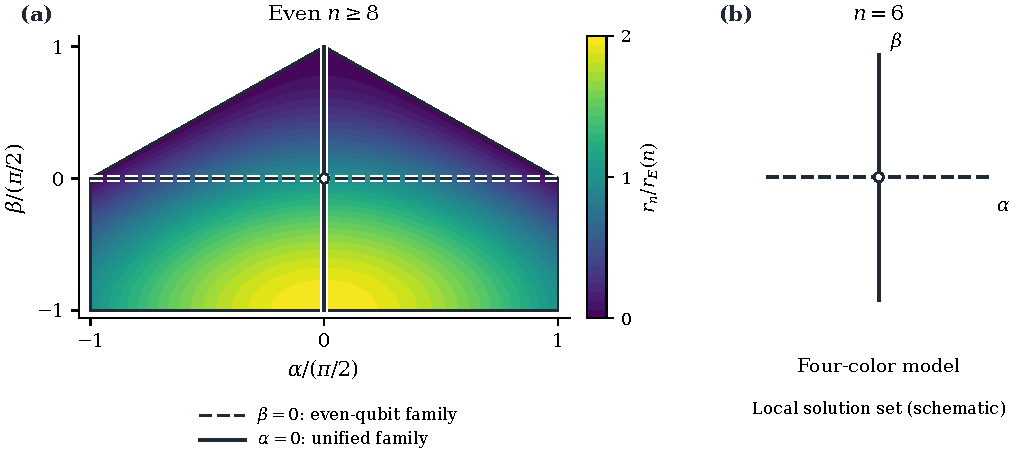
\includegraphics[width=\textwidth]{figures/fig2_embedding.pdf}
  \caption{偶数比特母族的两个精确截面。
  (a) 偶数 $n\geq8$ 的参数域 $\Omega$，颜色表示 $r_n/r_E(n)=\cos\alpha-\sin\beta$。
  虚线截面 $\beta=0$ 逐列恢复已知偶数族，实线截面 $\alpha=0$ 逐列恢复统一增强族。空心圆为共同基点。
  (b) $n=6$ 时四联合颜色加独立零点相位模型的局部解集示意：两支在基点交叉。 绘图代码由 OpenAI Codex（GPT-6）辅助编写，并按文中公式核对。}
  \label{fig:embedding}
\end{figure*}
